\chapter{PCB}

\section{Diseño físico} \label{DiseñoFisico}

Como ya se decidió en la sección \ref{Herramientas} y como ya se ha usado para el diseño esquemático, esta nos permitirá trasladar los componentes a un modelo físico de la placa base. Pero antes de poder mover los componentes a la placa, deberíamos saber a qué lugar van y de que forma. Por lo que antes de ponernos con el diseño de la placa deberemos diseñar el esquema físico del mismo. Para este apartado usaremos la herramienta AutoCad que se especifica en la sección \ref{Herramientas}.

Será necesario el diseño de las siguientes partes, \gls{PCB}, Carcasa, Disposición de teclas, ubicación de los componentes, ubicación de los conectores.

Estos diseños puede ser creados un mismo archivo de AutoCAD con las 3 vistas. Alzado, Perfil izquierdo y Planta. Esta última nos servirá para el diseño de la \gls{PCB} y de la disposición de teclas, así como poder crear el archivo 3D para la carcasa. Con el resto de vista nos serviremos para saber si el tamaño de los cortes y disposiciones de los elementos del teclado encajan entre sí y hay suficiente espacio para albergarlos en el interior de la carcasa.

El orden del diseño va a ser el siguiente. Disposición de teclas, diseño de la \gls{PCB}, diseño de la carcasa. Una vez tenemos esto podemos crear la \gls{PCB} en el programa EAGLE. El resto de los planos serán de confirmación y para asegurarnos de que lo que estamos haciendo saldrá correctamente.

\begin{tcolorbox}[colback=blue!5!white, colframe=blue!55!white, title=Nota]
    Ver el apéndice \ref{ApendicePCB} para más información sobre el diseño los planos y las consideraciones tomadas. 
\end{tcolorbox}

\newpage
\subsection{Diseño de la distribución} \label{CreacionPlanoDistribucion}

En el capítulo de diseño \ref{CapDiseño} en la sección \ref{DiseñoLayaout} se encontró una página web ''Plate \& Case Builder'' \cite{builder-swillkb} que nos generaba un plano para AutoCad basándonos en la distribución de teclas creada en la página web ''Keyboard Layout Editor'' \cite{Layout-Editor}.

Por lo que vamos a proceder a crear el plano primero para saber la distancia relativa entre las teclas y sus posiciones entre sí. Una vez introducido en ''\glsnocase{Plate} Layout'' el texto que nos genera la página del editor de distribución le damos a generar archivo CAD. Este nos genera el plano que podemos ver en la figura \ref{fig:PlanoDistribucionLayout}.

\begin{figure}[H]
    \centering
    \includegraphics[width=1\textwidth]{imagenes/Capitulos/Cap05/PlanoDiseñoTeclas.png}
    \caption{Imagen del plano generado por la página web ''Plate \& Case Builder'' \cite{builder-swillkb}}
    \label{fig:PlanoDistribucionLayout}
\end{figure}

\subsection{Medidas Físicas} \label{MedidasFisicas}

A partir del plano generado en la sección \ref{CreacionPlanoDistribucion} empezaremos a crear el resto de planos en AutoCad.

El primer paso es crear las dimensiones de la \gls{PCB}. Que en este caso van a ser el mínimo necesario para poder encajar todas las teclas y un borde de seguridad para que las \glsnocase{Keycaps} no toquen el borde de la madera.

En la figura \ref{fig:PlanoSeparacionMadera} podemos ver en rojo el borde de la \gls{PCB} y la línea más próxima en negro la madera. Se ha dejado medio milímetro de margen para las máquinas \gls{CNC} y de fabricación de \gls{PCB}. Los marcadores de los interruptores generados por el software de la sección \ref{CreacionPlanoDistribucion} se ha dejado en verde.

También para obtener el plano de la \gls{PCB} es necesario añadir los tornillos, ya que como se diseñó en la sección \ref{DiseñoPlatePCB} y se decidió que el montaje del teclado iba a ser sin \glsnocase{Plate} como en la figura \ref{fig:Montaje7}, la fuerza de las manos presionando las teclas va a ser transmitida directamente a la \gls{PCB}. Esta fuerza hará que se doble fácilmente por el material del que está fabricada, que es menos rígido que las \glsnocase{Plate} convencionales. Se van a necesitar varios tornillos distribuidos a lo largo de toda la \gls{PCB} para poder hacer un teclado robusto.

Una vez que se ha importado el plano generado de las posiciones de los interruptores se va a proceder a quitar algunos elementos innecesario de marcado y simplificar algunos elementos del plano generado. Una vez hecho esto y ajustado las dimensiones para que cumplan con la decisión tomada en la figura \ref{fig:PlanoSeparacionMadera}. Se va a proceder a colocar los agujeros de los tornillos.

Los tornillos van a ser de 3 mm o los llamados M3. Estos son de un tamaño adecuado para que puedan ser ubicados entre las juntas de las teclas y en los bordes. Por lo que se dispondrán circunferencias a lo largo del plano en purpura indicando las posiciones de los agujeros que además serán los tornillos ciegos de las carcasa en un futuro. Una vez hecho esto nos quedamos con 25 tornillos y en la disposición final que podemos ver en el plano de la \gls{PCB} en la figura \ref{fig:PlanoPCB}.

El teclado va a necesitar otro tipo de agujeros para sujetar un difusor de luz para los \glsnocase{LED}s. Por lo que Vamos a tener que idear la posición de los \glsnocase{LED}s y además añadir los agujeros específicos para sujetar el difusor. Ya que vamos a colocar los \glsnocase{LED}s vamos a aprovechar y también colocar los planos de los diferentes componentes. Vamos a añadir el \glsnocase{Multiplexor}, el ESP32-S3, y el conector XS-12 y la pantalla que se habían decidido colocar en la sección \ref{DiseñoHardware}. Los agujeros para los \glsnocase{LED}s estarán marcados en azul y los componentes en naranja.

Una vez añadidos al plano todos los componentes importantes, la pantalla y haber marcado todos los agujeros que necesita la \gls{PCB} nos queda, por fin, el plano completo de la \gls{PCB} con todas las medidas correctas y en su lugar correspondiente. El plano se puede ver en la figura \ref{fig:PlanoPCBConTodo}.

\begin{figure}[H]
    \centering
    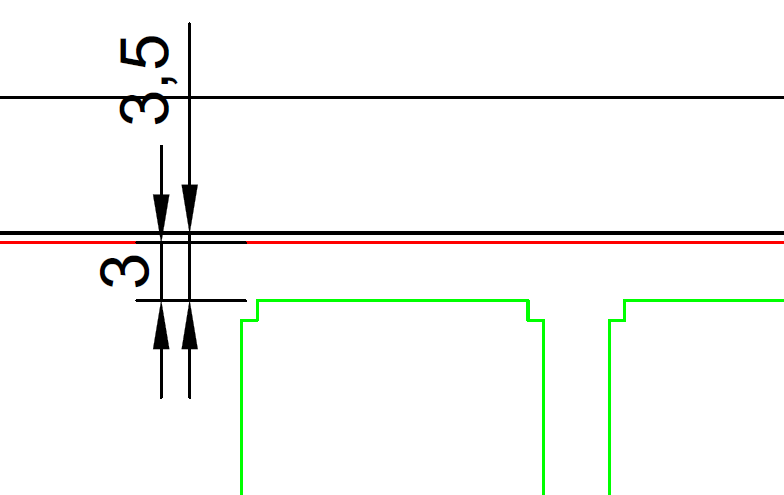
\includegraphics[width=0.8\textwidth]{imagenes/Capitulos/Cap05/AcotadoPCBMadera.png}
    \caption{Imagen del plano acotado del espacio entre las \glsnocase{Keycaps} y la madera.}
    \label{fig:PlanoSeparacionMadera}
\end{figure}

\begin{figure}[H]
    \centering
    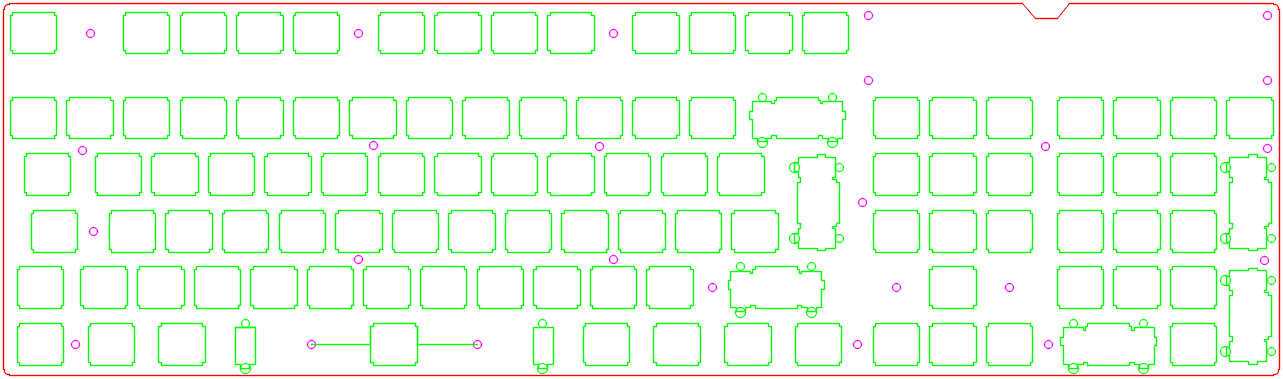
\includegraphics[width=1\textwidth]{imagenes/Capitulos/Cap05/PlanoPCB.png}
    \caption{Imagen del plano de la \gls{PCB}}
    \label{fig:PlanoPCB}
\end{figure}

\begin{figure}[H]
    \centering
    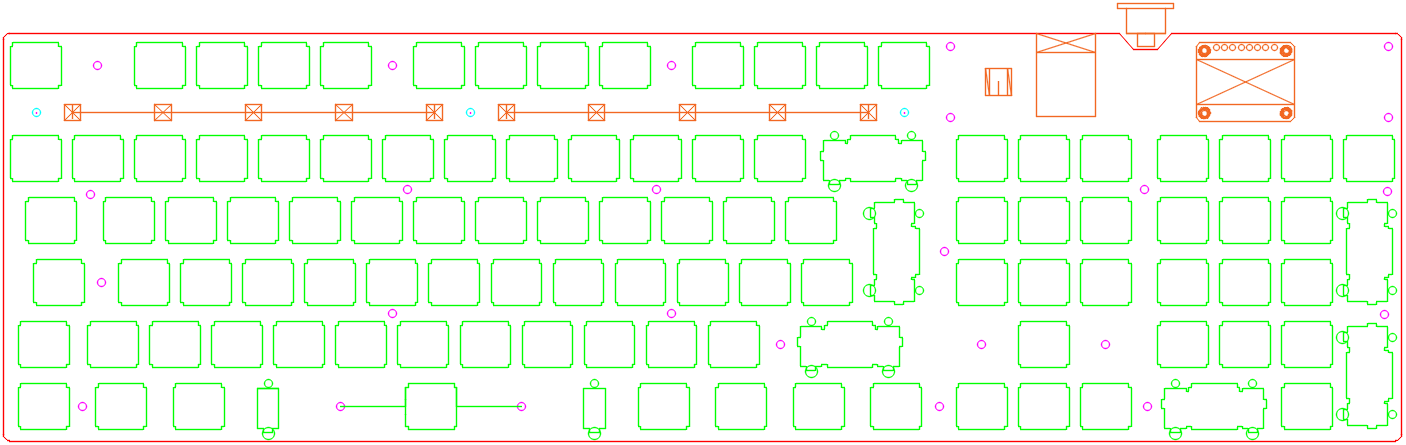
\includegraphics[width=1\textwidth]{imagenes/Capitulos/Cap05/PlanoConPartes.png}
    \caption{Imagen del plano completo de la \gls{PCB}}
    \label{fig:PlanoPCBConTodo}
\end{figure}

\subsection{Creación de la placa en Eagle}

Para la creación de la placa o del archivo necesario para poder encargar la placa por internet, vamos a volver a la herramienta Eagle, dado que ya tenemos el diseño esquemático completo hecho. Gracias a los componentes que hemos buscado en internet podremos hacer la parte física de una forma sencilla. Estos componentes tienen la información de como es la pieza física, por lo que si nos vamos al plano podemos encontrar todas las piezas dispersadas como se ve en la figura \ref{fig:EaglePCBNueva}.

Para poder colocar estos componentes en su lugar adecuado, tendremos que importar el plano que hicimos en AutoCAD. Lo guardaremos como .DXF y en Eagle le daremos a importar dxf. Una vez importado el plano nos aparecerá una capa nueva llamada documentación como se puede ver en la figura \ref{fig:EaglePCBPlano}. En esta capa estará albergado el plano de la \gls{PCB}. Ahora la tarea pendiente es colocar los elementos y componentes a lo largo de todo el plano siguiendo el orden correspondiente.

Una vez colocados todos los elementos nos quedará listo para empezar a conectar todo con los llamados líneas aéreas que son, simplemente, líneas amarillas que nos indican a donde tiene que ir la vía de conexión. Esto lo podemos ver en la figura \ref{fig:EaglePCBPartesColocadas}. 

Además, en la misma figura \ref{fig:EaglePCBPartesColocadas} ya hemos añadido los agujeros a la placa en sus correspondientes lugares. Además de dimensionar la capa de \gls{PCB} que nos dará la dimensión de la misma. Los agujeros se han realizado con la herramienta de ''Drill'' que nos permite localizar un taladro en el lugar que lo pongamos del tamaño que le indiquemos. También hemos creado las líneas de la capa ''dimensión'' que nos indica como debe ser la \gls{PCB} estas han sido colocadas siguiendo el borde rojo de la figura \ref{fig:PlanoPCBConTodo} en el plano de Eagle.

\begin{figure}[H]
    \centering
    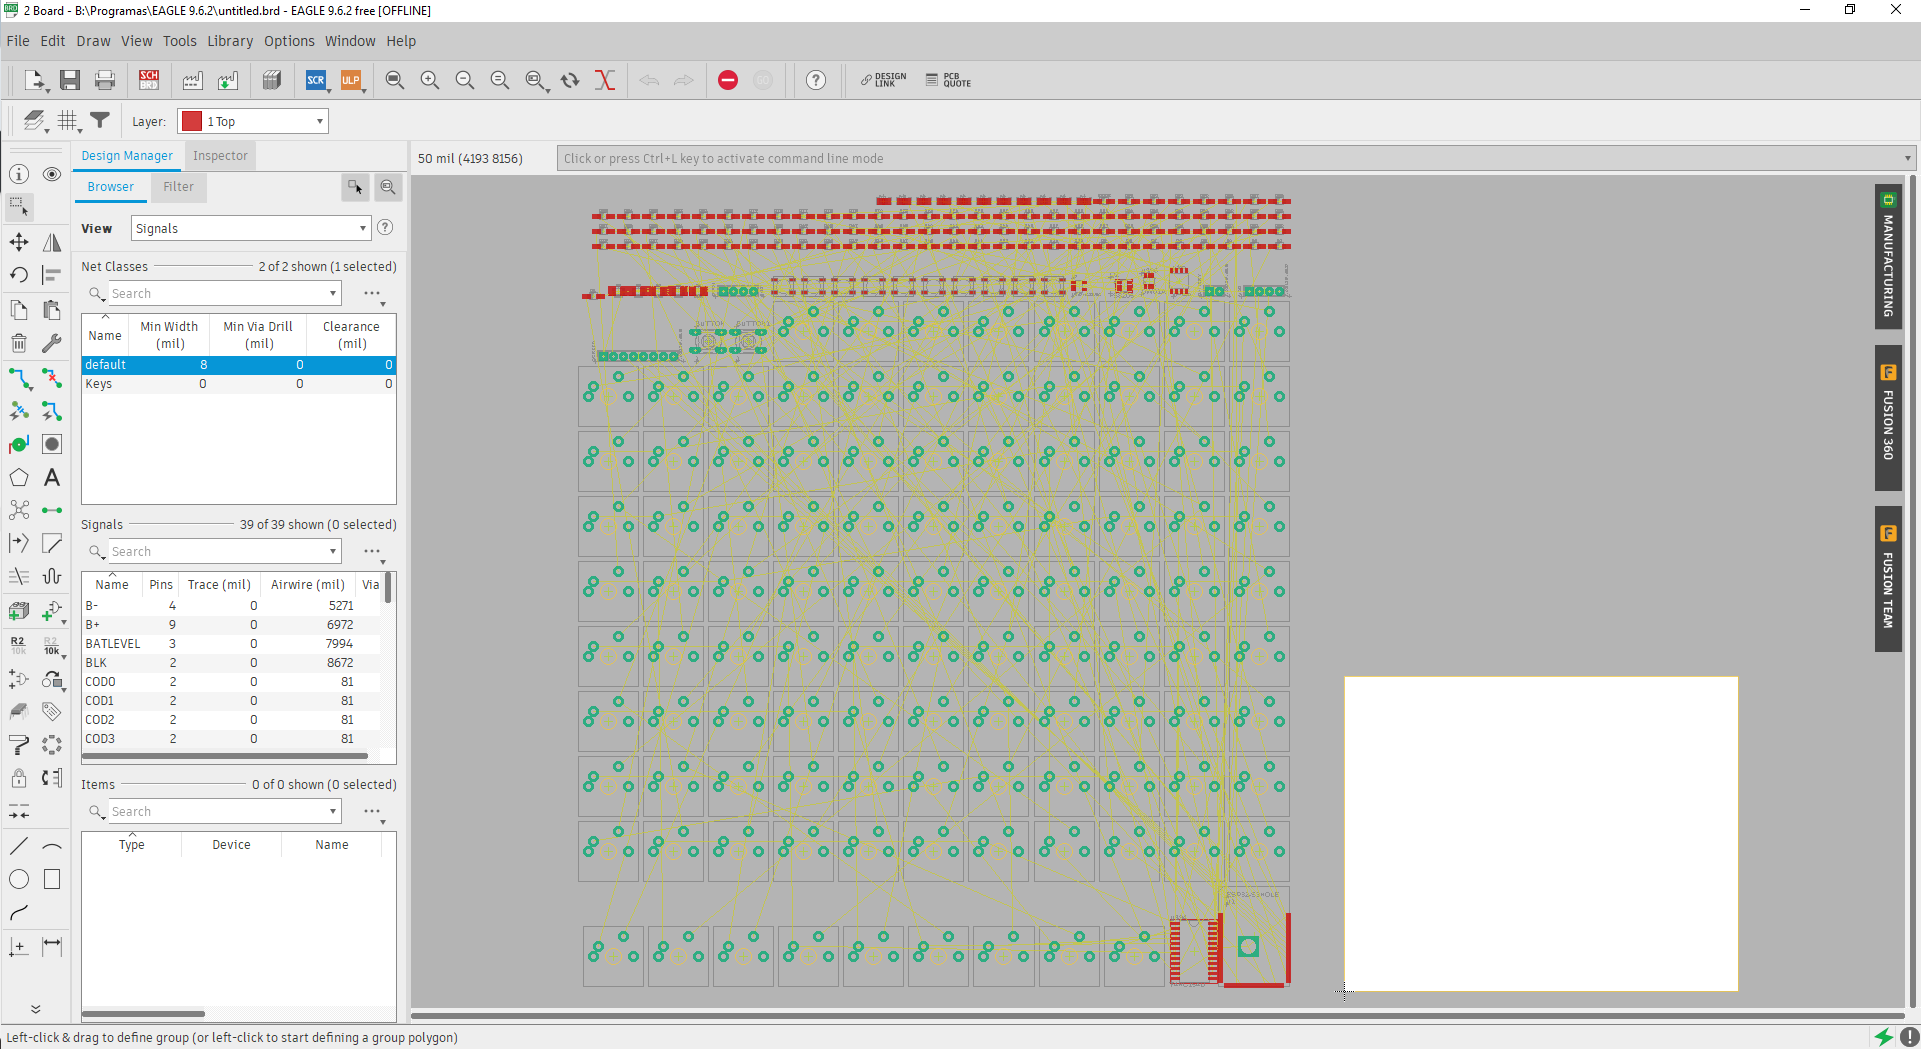
\includegraphics[width=1\textwidth]{imagenes/Capitulos/Cap05/EaglePCBNueva.png}
    \caption{Imagen de la vista \gls{PCB} en Eagle.}
    \label{fig:EaglePCBNueva}
\end{figure}

\begin{figure}[H]
    \centering
    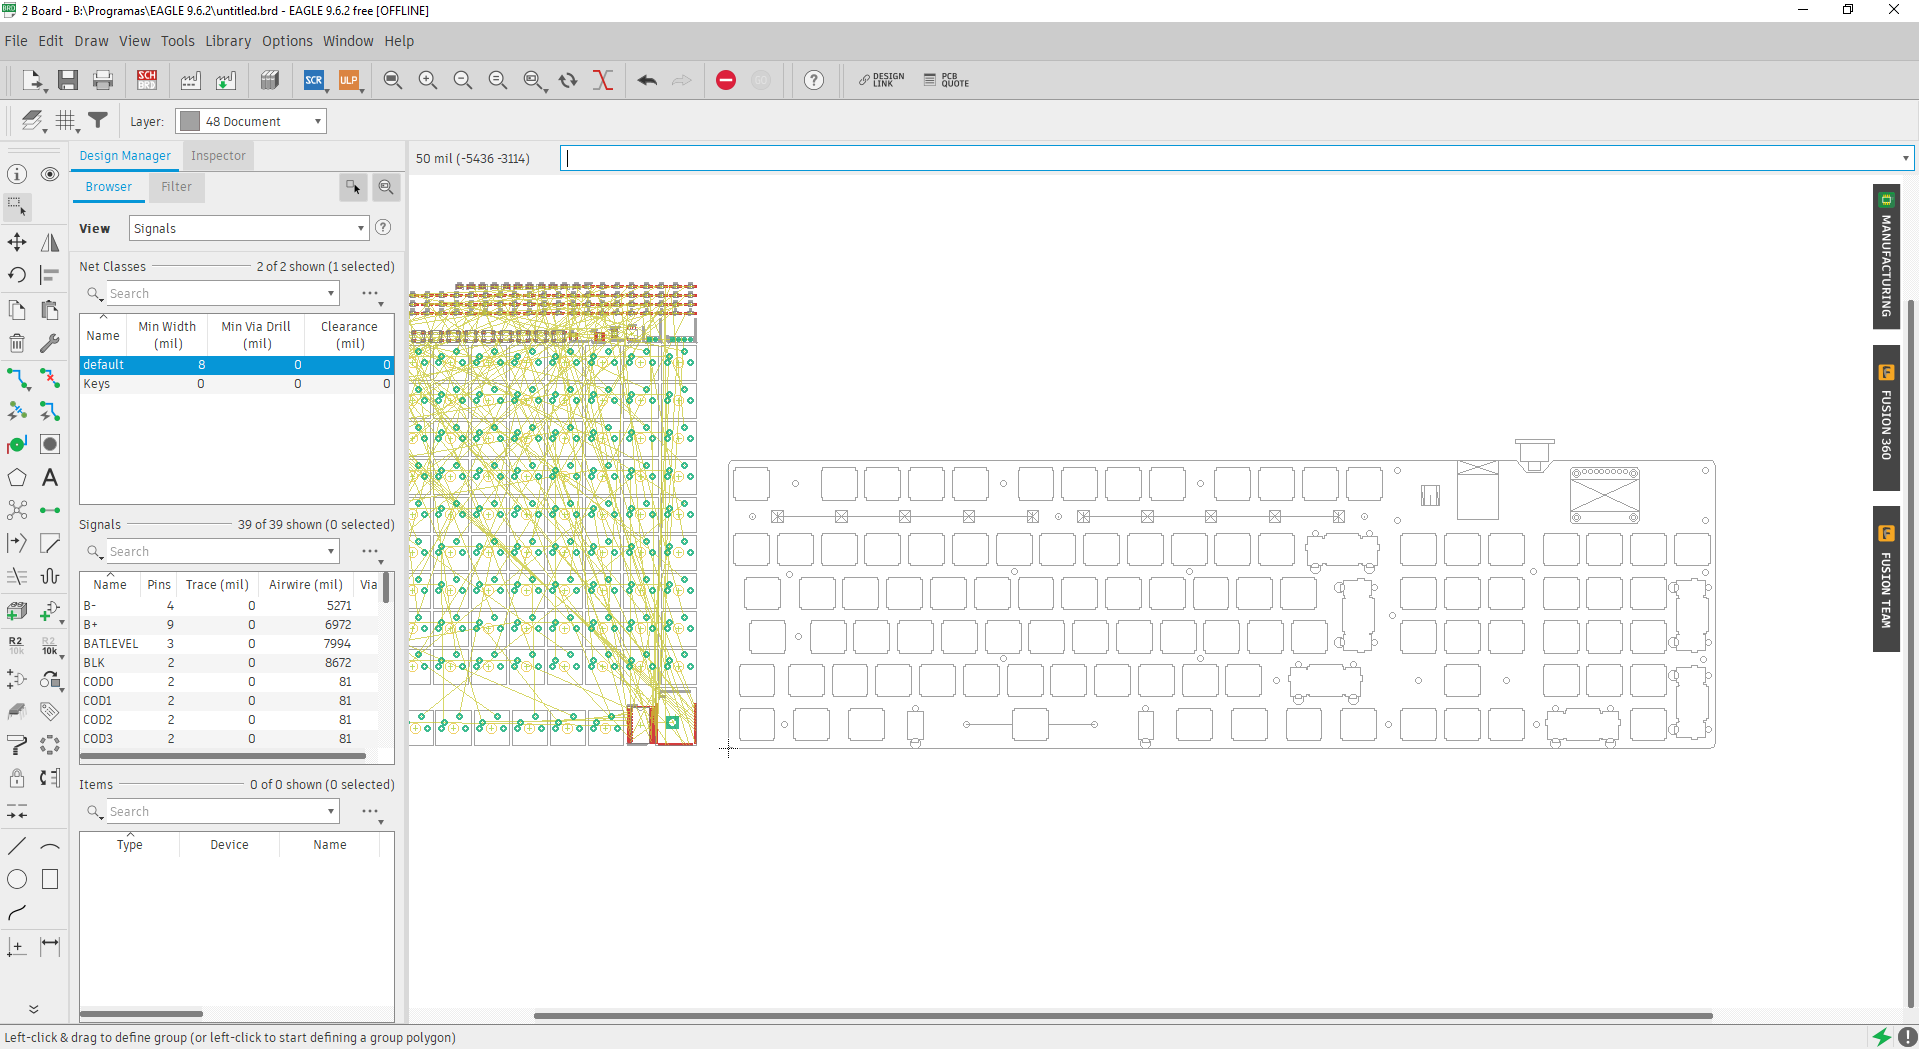
\includegraphics[width=1\textwidth]{imagenes/Capitulos/Cap05/EaglePCBPlano.png}
    \caption{Imagen del plano importado en Eagle.}
    \label{fig:EaglePCBPlano}
\end{figure}

\begin{figure}[H]
    \centering
    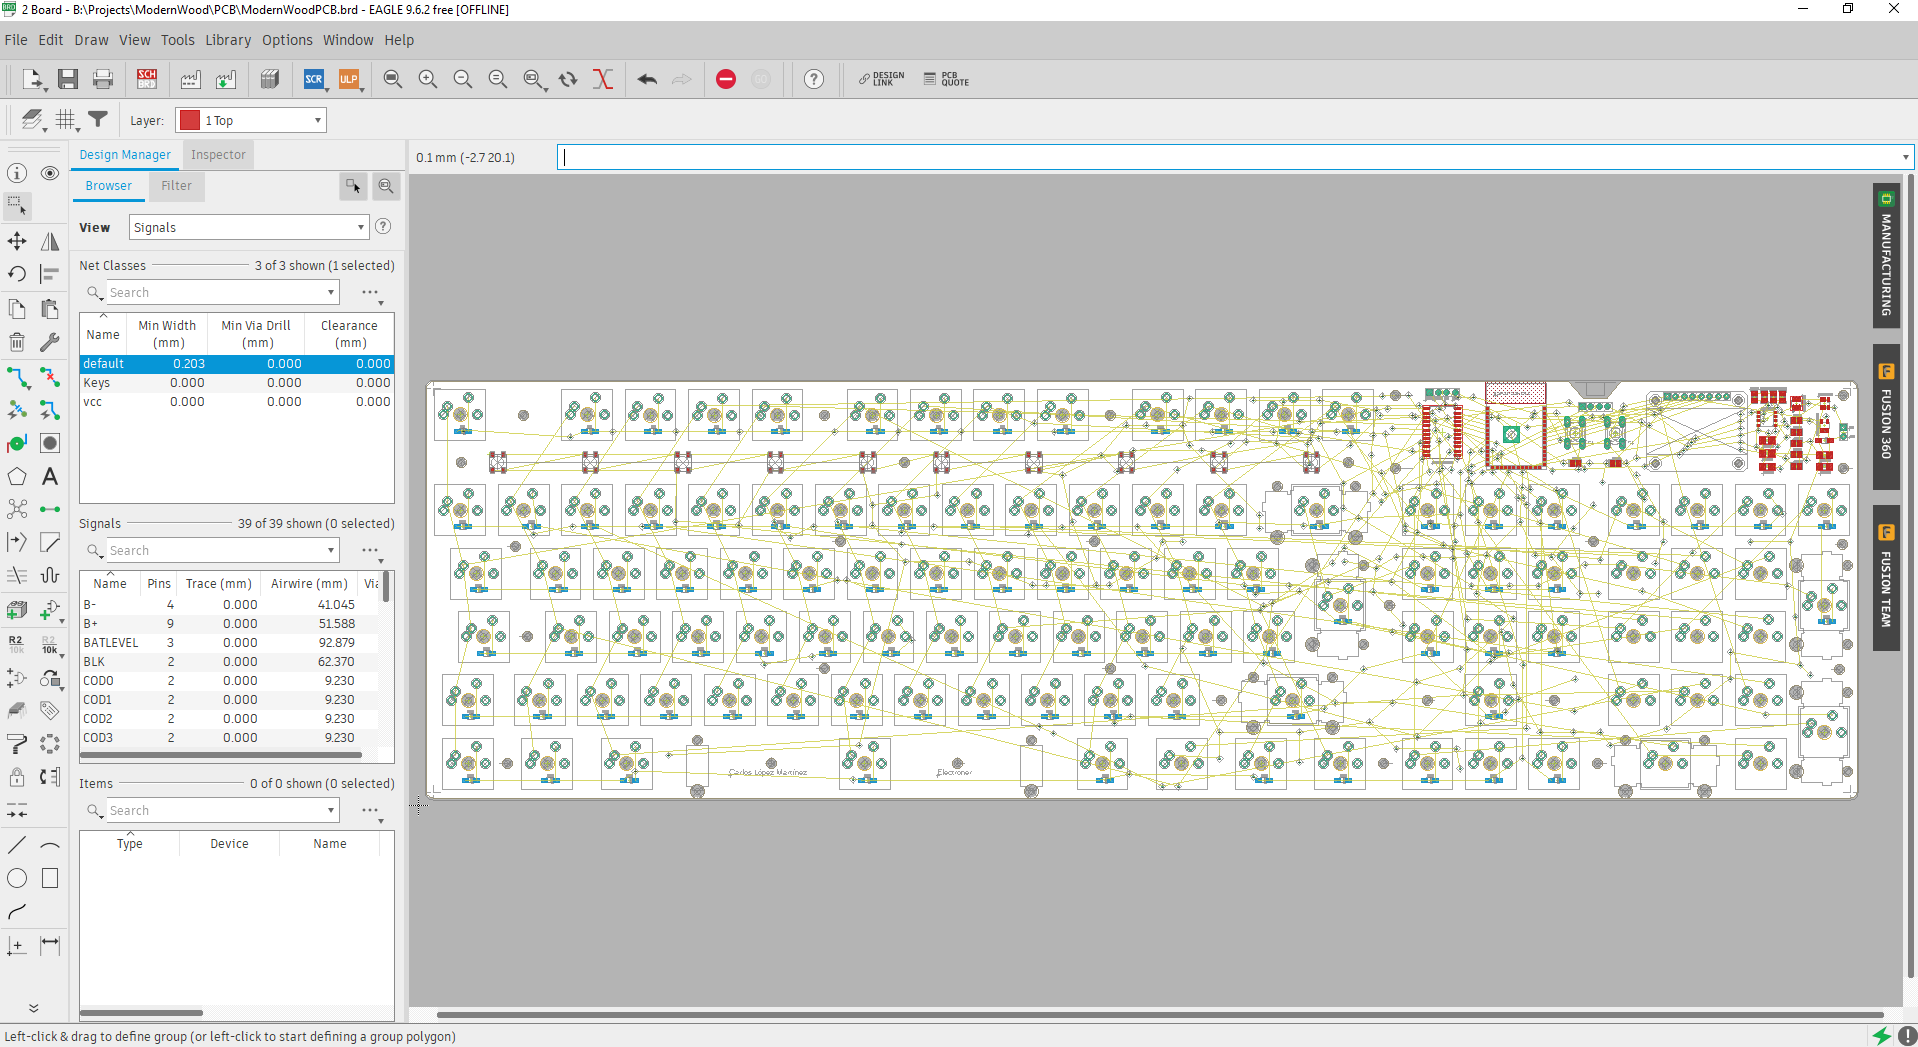
\includegraphics[width=1\textwidth]{imagenes/Capitulos/Cap05/EaglePCBPartesColocadas.png}
    \caption{Imagen de la \gls{PCB} con los componentes ubicados y los agujeros.}
    \label{fig:EaglePCBPartesColocadas}
\end{figure}

\subsubsection{Consideraciones de potencia y diseño}
Durante el diseño ha sido fundamental prestar atención a los voltajes de funcionamiento de las diferentes partes del teclado, ya que hay varios niveles de voltaje en todo el proyecto. Pero estas consideraciones también tiene que estar presentes ahora. Ya que durante el enrutamiento que vamos a realizar a continuación. Las pistas/carriles o vías que creemos tienen que cumplir unas características para el correcto funcionamiento del dispositivo.

En primer lugar, se debe prestar especial atención al dimensionamiento de los carriles de alimentación y conexión entre los distintos componentes del teclado. Los carriles deben tener el tamaño adecuado para manejar la corriente requerida por los componentes sin causar caídas de tensión significativas que puedan afectar al rendimiento del teclado.

Además, la posición de los elementos de potencia y otros componentes críticos debe ser cuidadosamente considerada. Una disposición incorrecta puede resultar en interferencias electromagnéticas (EMI) o en problemas de disipación de calor, lo que podría afectar negativamente al funcionamiento del teclado y su durabilidad.

Para ello vamos a usar herramientas de cálculo de pistas o vías para saber qué características tienen que tener. Vamos a calcular que distancia mínima y que tamaño tienen que tener las pistas. Para ello vamos a usar dos páginas que tienen calculadoras específicas para realizar esta tarea.

El primer valor va a ser el tamaño de la vía, para ello vamos a usar la página ''4pcb'' \cite{4pcbCalculator} y para la distancia entre pistas ''protoexpress'' \cite{protoexpressCalculator}. 

Empecemos con el tamaño de la vía, los parámetros que nos pide son los siguientes.
\begin{itemize}
    \item \textbf{Intensidad}. Este valor para nosotros va a valer como máximo 0,5 Amperios, ya que es el máximo que el \gls{USB} nos da.
    \item \textbf{Grosor}. Este valor es un estándar, así que para nosotros es de 2 $\frac{oz}{ft^2}$.
    \item \textbf{Temperatura}, Incremento y ambiente. Nuestra temperatura ambiente será de 25ºC y el incremento le pondremos de otros 25.
    \item \textbf{Longitud de la pista}. La distancia. Aquí vamos a elegir la pista más larga en nuestro teclado que será de lado a lado de unos 50 cm.
\end{itemize}

El resultado que nos arroja esta calculadora es de un grosor de 0.0861 mm. Como podemos ver, el tamaño de la pista es sumamente pequeño, por lo que los valores por defecto de Eagle nos van a valer perfectamente y además mejorara la resistencia y la caída de voltaje.

Para la distancia de la pista los parámetros que nos piden son:
\begin{itemize}
    \item \textbf{Máximo voltaje de la pista}. Para nosotros el voltaje más alto que tenemos en todo el circuito es de 5V (Entrada del \gls{USB}).
\end{itemize}

Tras darle a calcular, el valor que obtenemos es de 0,0508 mm. Otra vez los valores por defecto del programa superan con creces este valor. Por lo que por ahora cumplimos con todos los requisitos.

Cabe mencionar, que dado que el microcontrolador ESP32S3 es el que posee la antena \gls{Bluetooth} integrada, no es necesario calcular nada relacionado con la antena. Ya que el fabricante del microcontrolador ya ha hecho este trabajo por nosotros.

\subsubsection{Enrutamiento}
%explicar que se ha hecho de forma automatica la seccion de las teclas y se ha revisado a mano. Y mencionar que la seccion de micro ha sido hecha a mano
Para la sección de las teclas se ha usado la herramienta de enrutamiento automático de Eagle. Esta herramienta nos permite conectar todas las pistas de forma rápida y eficiente. Una vez que se ha realizado el enrutamiento automático, se ha revisado manualmente para asegurarse de que todas las conexiones son correctas y que no hay errores en el diseño.

Para la sección del microcontrolador y los componentes críticos, se ha realizado el enrutamiento manualmente. Esto se debe a que estas secciones son más críticas y requieren una mayor atención para asegurarse de que todas las conexiones son correctas y que no hay curvas extrañas que puedan afectar al rendimiento del teclado.

Una vez conectado todo nos quedaría la \gls{PCB} terminada. La podemos ver en la figura \ref{fig:EaglePCBConectada}. En esta figura podemos ver que todas las pistas están conectadas y que todos los componentes están en su lugar correspondiente. Además, se han añadido las pistas de alimentación y las pistas de conexión entre los diferentes componentes.

%Mencionar el plano de tierra que hemos creado para mejorar el ruino de la placa. Y que siempre es recomendable tener un plano de tierra en la placa.
Además de conectar todos los componentes, se ha añadido un plano de tierra en la \gls{PCB}. Este plano de tierra ayuda a mejorar la disipación del calor y a reducir las interferencias electromagnéticas (EMI) en la placa. También ayuda a mejorar la integridad de la señal y a reducir el ruido en la placa. Por lo que siempre es recomendable tener un plano de tierra en la placa. Se ha creado un plano para cada una de las capas de la \gls{PCB}. Como nosotros tenemos 2 capas, hemos creado un plano de tierra en la capa superior y otro en la capa inferior.
Estos planos se pueden ver en la figura \ref{fig:EaglePCBPlanoTierra1} y en la figura \ref{fig:EaglePCBPlanoTierra2}, respectivamente.

\begin{figure}[H]
    \centering
    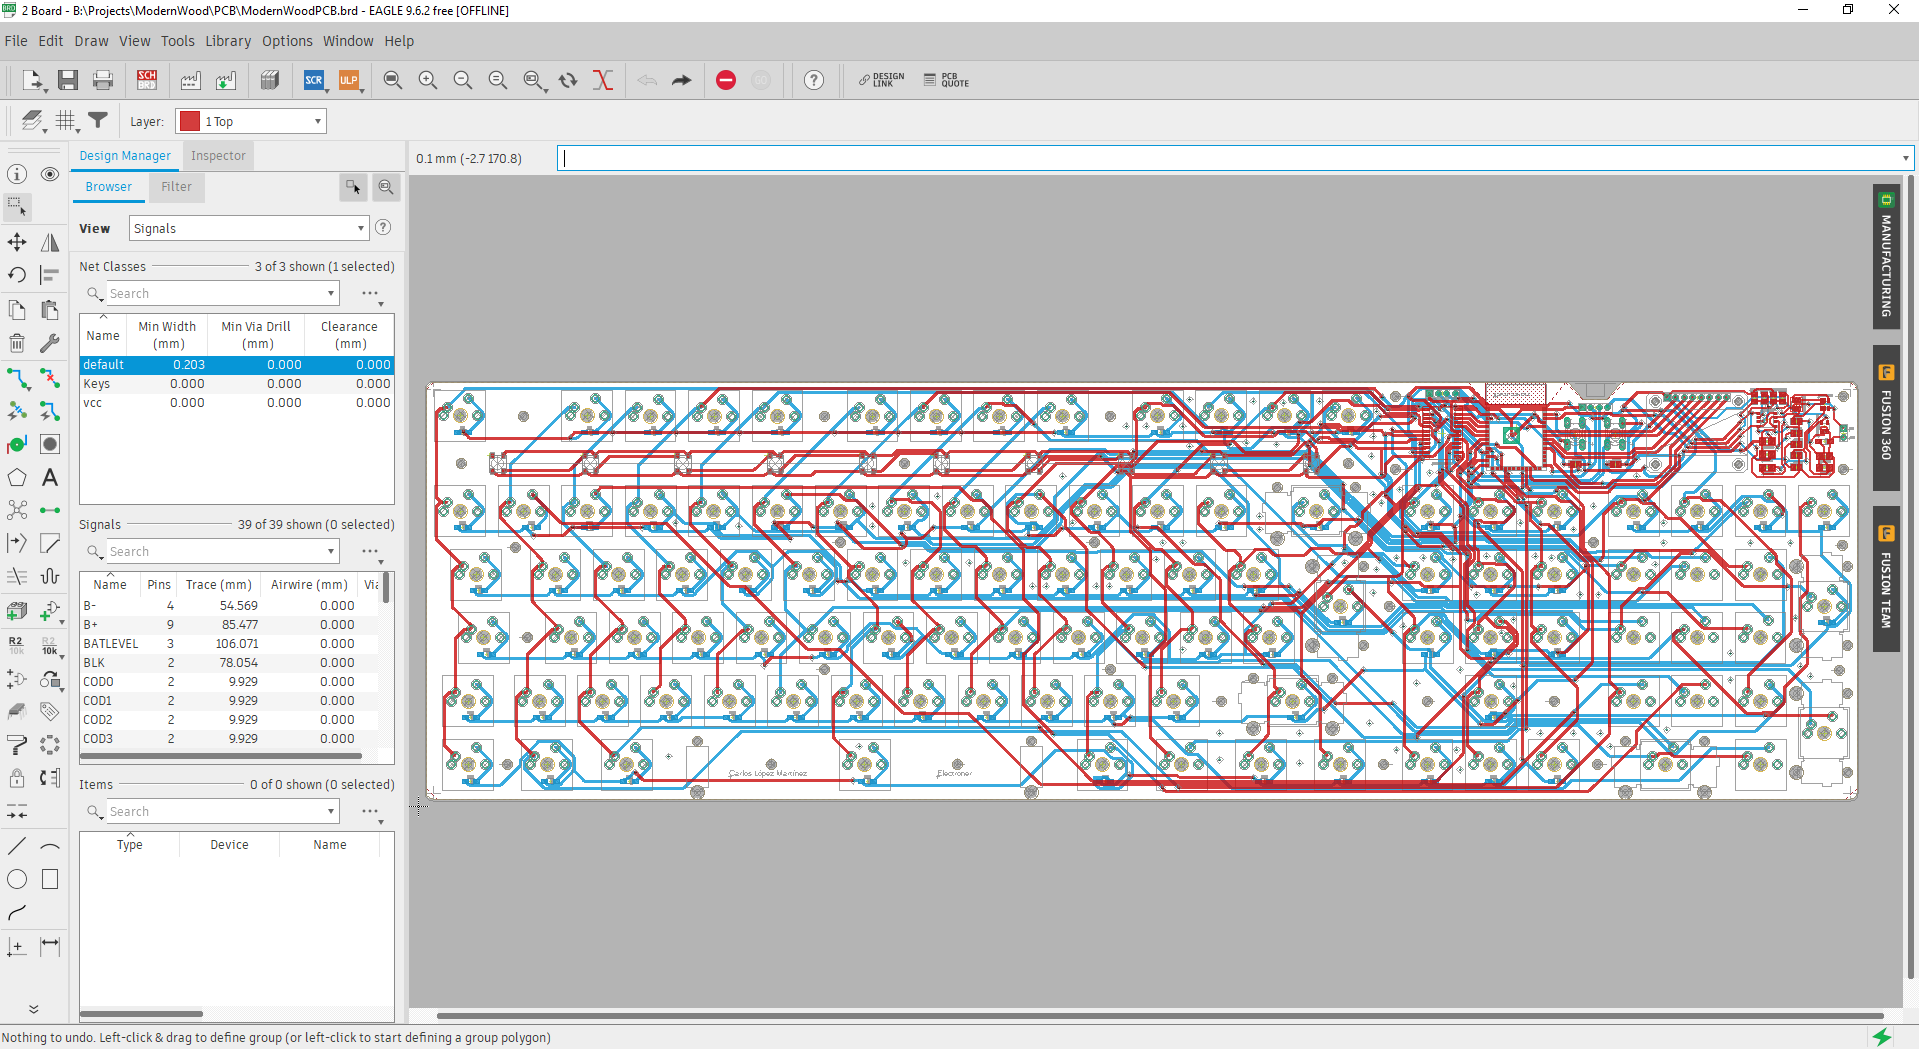
\includegraphics[width=1\textwidth]{imagenes/Capitulos/Cap05/EaglePCBConectada.png}
    \caption{Imagen de la \gls{PCB} con las pistas conectadas.}
    \label{fig:EaglePCBConectada}
\end{figure}

\begin{figure}[H]
    \centering
    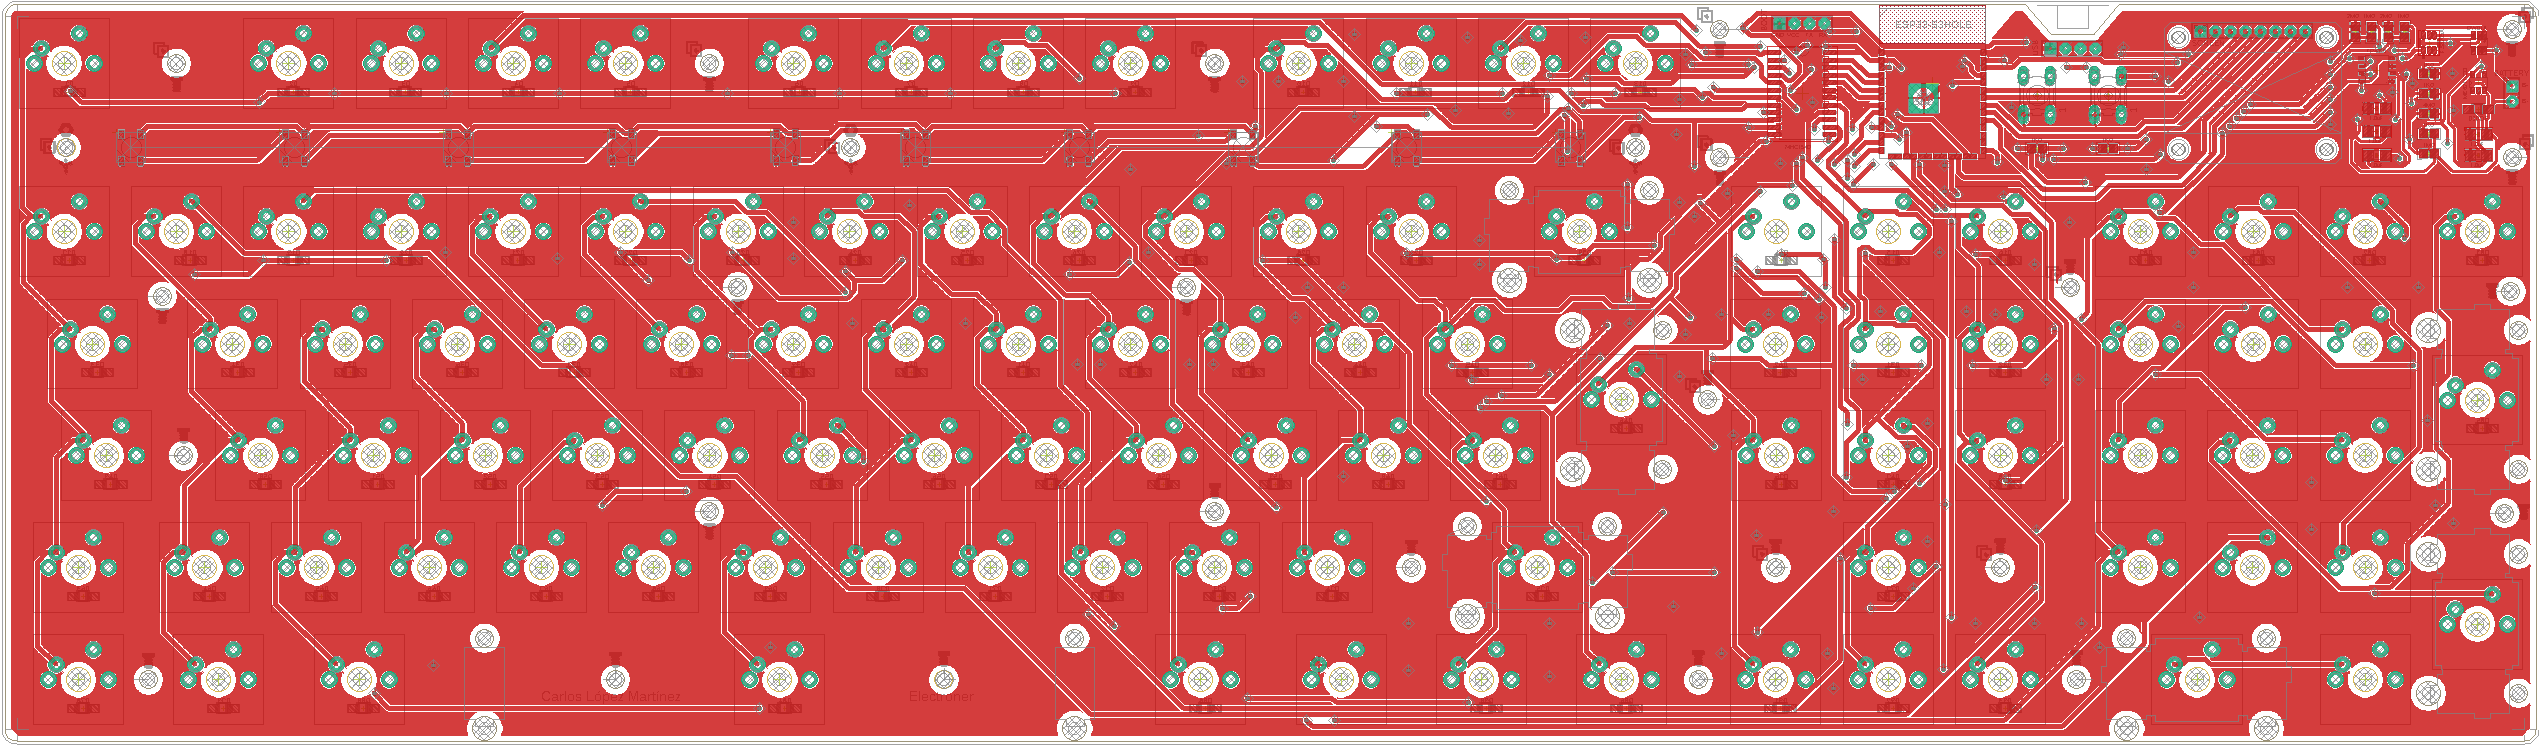
\includegraphics[width=1\textwidth]{imagenes/Capitulos/Cap05/EaglePCBPlanoTierra1.png}
    \caption{Imagen del plano de tierra superior de la \gls{PCB}.}
    \label{fig:EaglePCBPlanoTierra1}
\end{figure}

\begin{figure}[H]
    \centering
    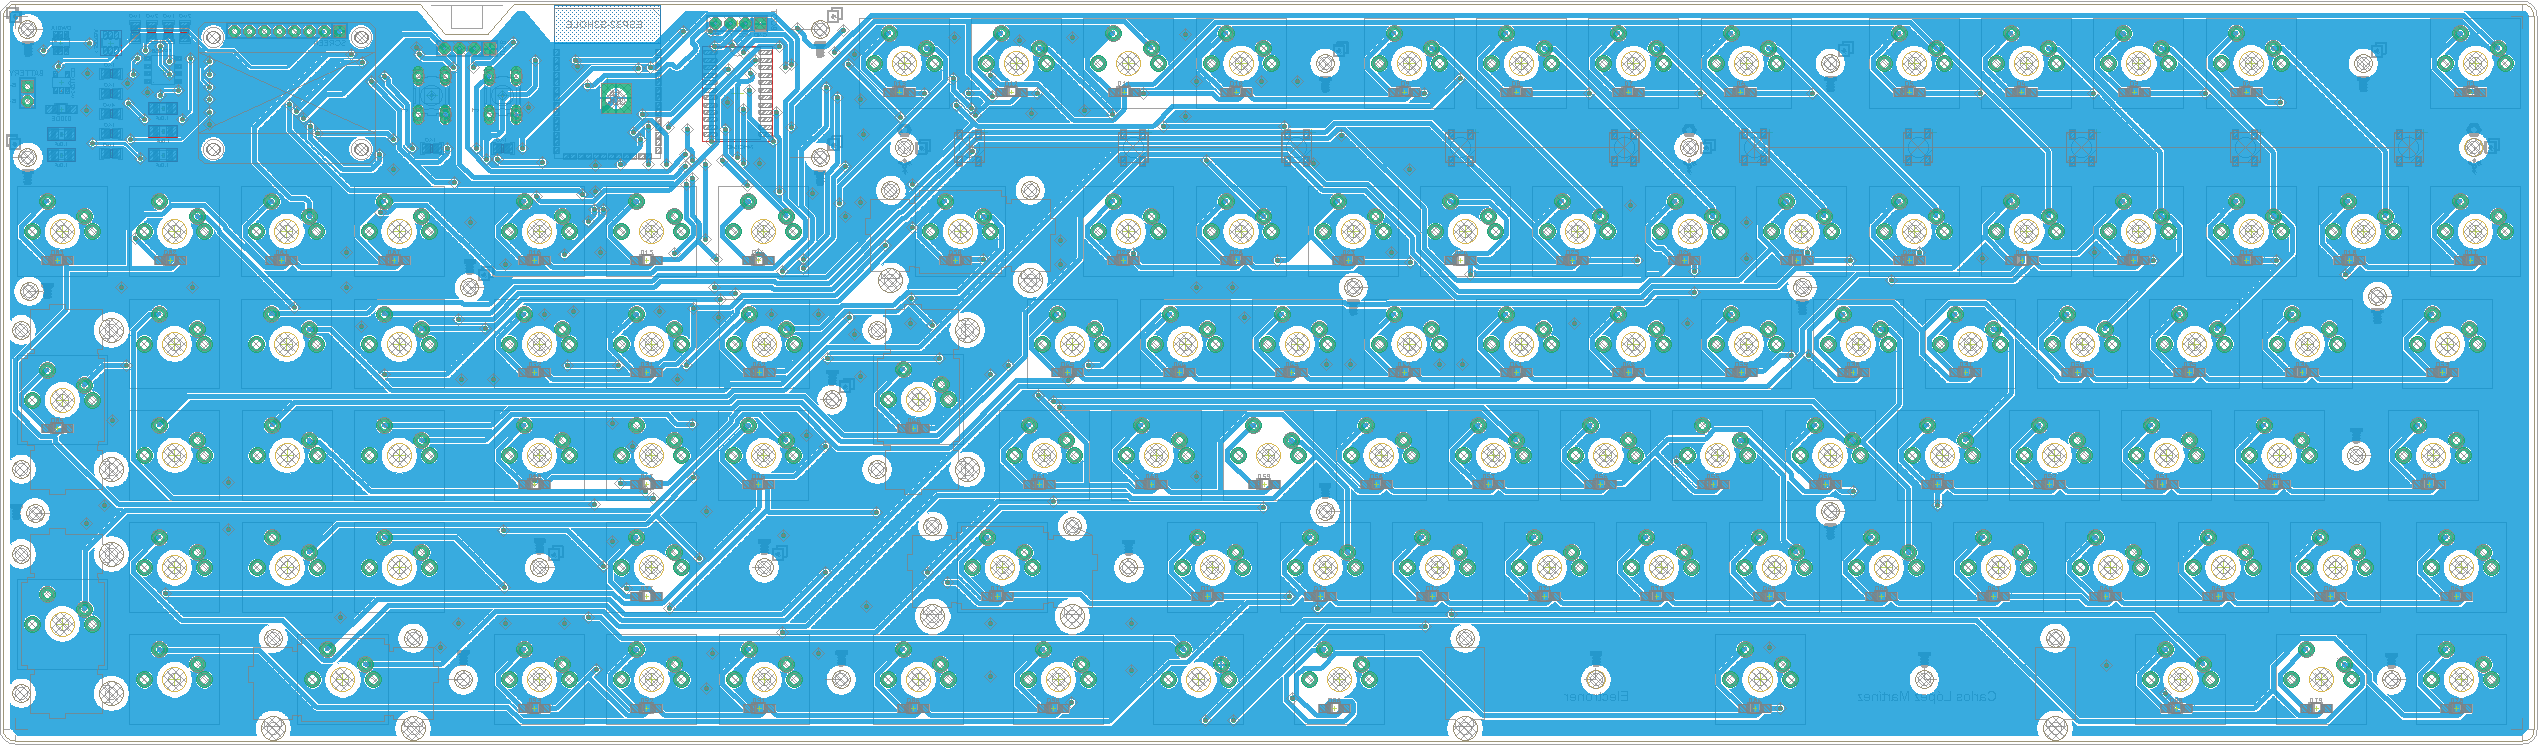
\includegraphics[width=1\textwidth]{imagenes/Capitulos/Cap05/EaglePCBPlanoTierra2.png}
    \caption{Imagen del plano de tierra inferior de la \gls{PCB}.}
    \label{fig:EaglePCBPlanoTierra2}
\end{figure}

\subsubsection{Estética}
%Quitar las marcas de las Vias entre otras, poner el texto a mano, indicadores, POsicionar todo correctamente. Mover las vias para que queden más estetias etc.
Una vez que se ha realizado el enrutamiento y se han añadido los planos de tierra, se ha procedido a mejorar la estética de la \gls{PCB}. Para ello, se han eliminado las marcas de las vías y se han movido las vías para que queden más estéticas. También se ha añadido el texto a mano y se han posicionado todos los elementos de forma correcta. Además, se han añadido indicadores para facilitar la lectura de la \gls{PCB} y se han añadido los números de referencia de los componentes para facilitar la identificación de los mismos.

A su vez, también se han creado unos iconos para poder identificar los tipos de agujeros a los que están asociados. En total hay 4 iconos. Estos son para identificar el difusor de luz, cuáles tienen un panel de metacrilato para poder proteger la sección de componentes electrónicos, otro para saber cuál es necesario emplear tuerca y el último para saber cuál es necesario atornillar a la carcasa. Respectivamente, estos iconos podemos previsualizarlos en las figuras \ref{fig:difusionIcono}, \ref{fig:MetacrilatoIcono}, \ref{fig:TuercaIcono} y \ref{fig:TornilloIcono} respectivamente.

Más adelante se usarán para saber de forma rápida que tipo de agujero es necesario en la carcasa. Y para facilitar el montaje del teclado.

\begin{itemize}
    \item \textbf{Difusor de luz}. 
    \begin{figure}[H]
        \centering
        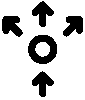
\includegraphics[width=0.15\textwidth]{imagenes/Capitulos/Cap05/Difusion.png}
        \caption{Imagen del icono de difusor de luz.}
        \label{fig:difusionIcono}
    \end{figure}
    \newpage
    \item \textbf{Panel de metacrilato}. 
    \begin{figure}[H]
        \centering
        
\includegraphics[width=0.15\textwidth]{imagenes/Capitulos/Cap05/Glass.png}
        \caption{Imagen del icono del indicador de panel de metacrilato.}
        \label{fig:MetacrilatoIcono}
    \end{figure}
    \item \textbf{Tuerca}. 
    \begin{figure}[H]
        \centering
        
\includegraphics[width=0.15\textwidth]{imagenes/Capitulos/Cap05/Nut.png}
        \caption{Imagen del icono del indicador de tuerca}
        \label{fig:TuercaIcono}
    \end{figure}
    \item \textbf{Atornillar a la carcasa}. 
    \begin{figure}[H]
        \centering
        
\includegraphics[width=0.1\textwidth]{imagenes/Capitulos/Cap05/Screw.png}
        \caption{Imagen del icono del indicador tornillo a la carcasa.}
        \label{fig:TornilloIcono}
    \end{figure}
\end{itemize}